% !TeX root = ../Tempel-Daniel.tex
\chapter{AI Agents and Agent Harnesses}
\label{chap:agents}

The previous chapters established the components required for the AI Software Engineering Assistant to construct context, retrieve repository information and request external operations through structured tool calls, which the runtime may route through MCP. These capabilities do not by themselves coordinate multiple actions toward a task objective.

A request such as \emph{Fix GitHub issue \#42 and verify the solution} may require inspection, modification, testing and further investigation based on intermediate results. In this report, an \textbf{agent} is a system in which an LLM selects actions toward a task objective, while an \textbf{agent harness} executes and constrains those actions, maintains operational state and returns observations for subsequent decisions.

\section{From tool calls to an agent loop}
\label{sec:agent-loop}

An \textbf{agent loop} extends the tool interaction described in Chapter~\ref{chap:tool-use} across a task. Figure~\ref{fig:agent-loop} shows how the harness constructs context, invokes the model, dispatches accepted actions and updates task state before deciding whether another iteration is permitted.

\begin{center}
\begin{minipage}{\linewidth}
\centering
\captionsetup{hypcap=false}
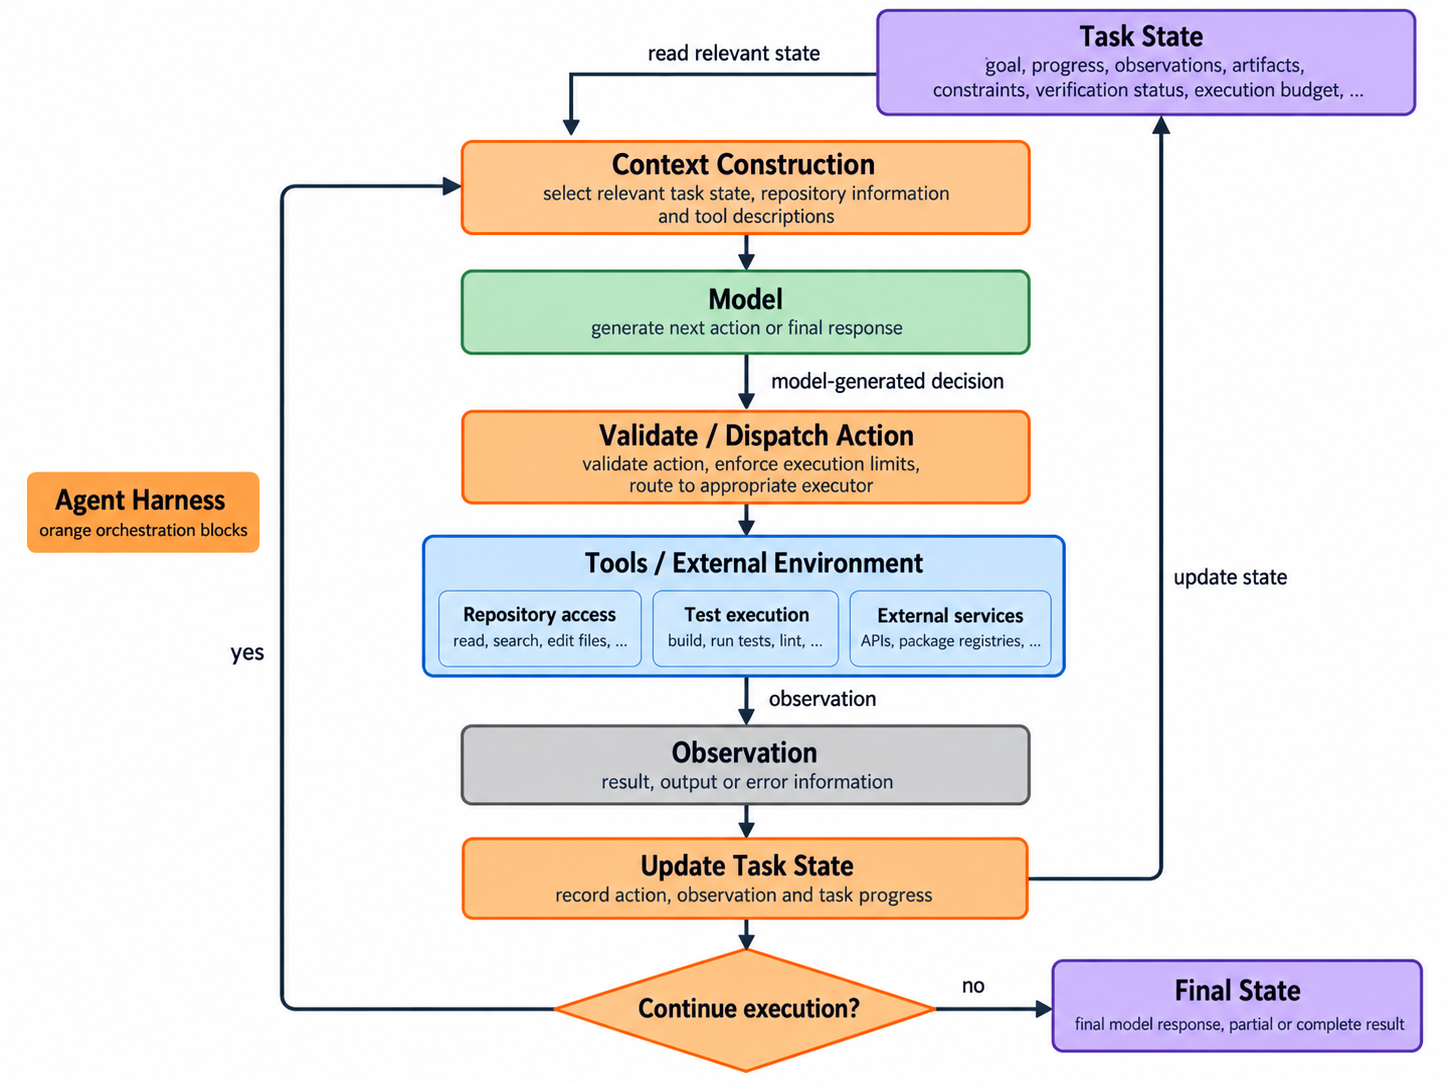
\includegraphics[width=\linewidth]{images/agent-loop-harness.png}
\captionof{figure}{Agent loop in which the model selects subsequent actions while the agent harness constructs context, dispatches actions, updates task state and controls continuation. Termination of the loop does not by itself establish successful task completion.}
\label{fig:agent-loop}
\end{minipage}
\end{center}

The return path supplies updated observations for the next model decision; leaving the loop does not itself establish task success. If \texttt{run\_tests} executes correctly but reports failing assertions, the result is a useful observation that may lead to further inspection or another modification. Failure to start the test process or a timeout instead represents an execution problem and may require runtime-level recovery.

A workflow may also branch according to intermediate results while following predefined orchestration rules. In the agent loop considered here, the model has greater freedom to select and sequence subsequent actions within limits enforced by the harness. Real systems can combine both approaches. Anthropic similarly distinguishes predefined workflows from agents that dynamically direct their own tool usage \parencite{schluntz2024agents}.

This interaction is related to the action–observation structure of ReAct, where external actions provide evidence for subsequent model decisions \parencite{yao2023react}. Interface design also matters. SWE-agent demonstrates through its \textbf{Agent-Computer Interface (ACI)} that the behaviour and feedback of repository navigation, editing and execution tools can materially affect agent performance \parencite{yang2024sweagent}.

\section{Task state, recovery and completion}
\label{sec:agent-task-state}

Multi-step execution requires a coherent \textbf{task state} independent of the active model context. Relevant state can include the task objective, progress, modified artefacts, observations, verification status and execution budget. Only the subset needed for the next decision has to enter the active context.

State should reflect its source. Execution and verification status should be updated from runtime-observed results: requesting \texttt{apply\_patch} does not mean that a file was modified, and a model statement that tests passed is not a verification result. Model-generated plans and root-cause hypotheses remain inferred information until supported by observations.

Failure handling occurs at different levels. A transient infrastructure problem may justify a bounded \textbf{runtime retry} of the same operation. A compiler error or failing assertion produced by a successfully executed tool instead becomes an observation for \textbf{model-driven recovery}, in which the model changes its strategy or gathers additional evidence.

Side-effecting operations require additional care. If \texttt{create\_pull\_request} succeeds but its response is lost, blindly repeating the request may create a duplicate. The runtime should determine the previous outcome when possible. If this cannot be established, task state should preserve the uncertainty and automatic repetition may need to stop.

The harness also enforces execution budgets and stopping policies. When the model signals completion, the harness records whether available evidence satisfies the defined acceptance criteria. Missing or failed verification must remain distinguishable from verified completion. Longer tasks may additionally use checkpoints so that execution can resume after interruption; production persistence is addressed in the following chapter.

\section{Delegation and subagents}
\label{sec:agent-delegation}

A \textbf{subagent} is an additional agent assigned a bounded delegated task and a selected context. For issue \#42, Figure~\ref{fig:agent-delegation} shows parallel investigation of tests, code and recent changes, followed by integration, modification and verification by the main agent.

\begin{center}
\begin{minipage}{\linewidth}
\centering
\captionsetup{hypcap=false}
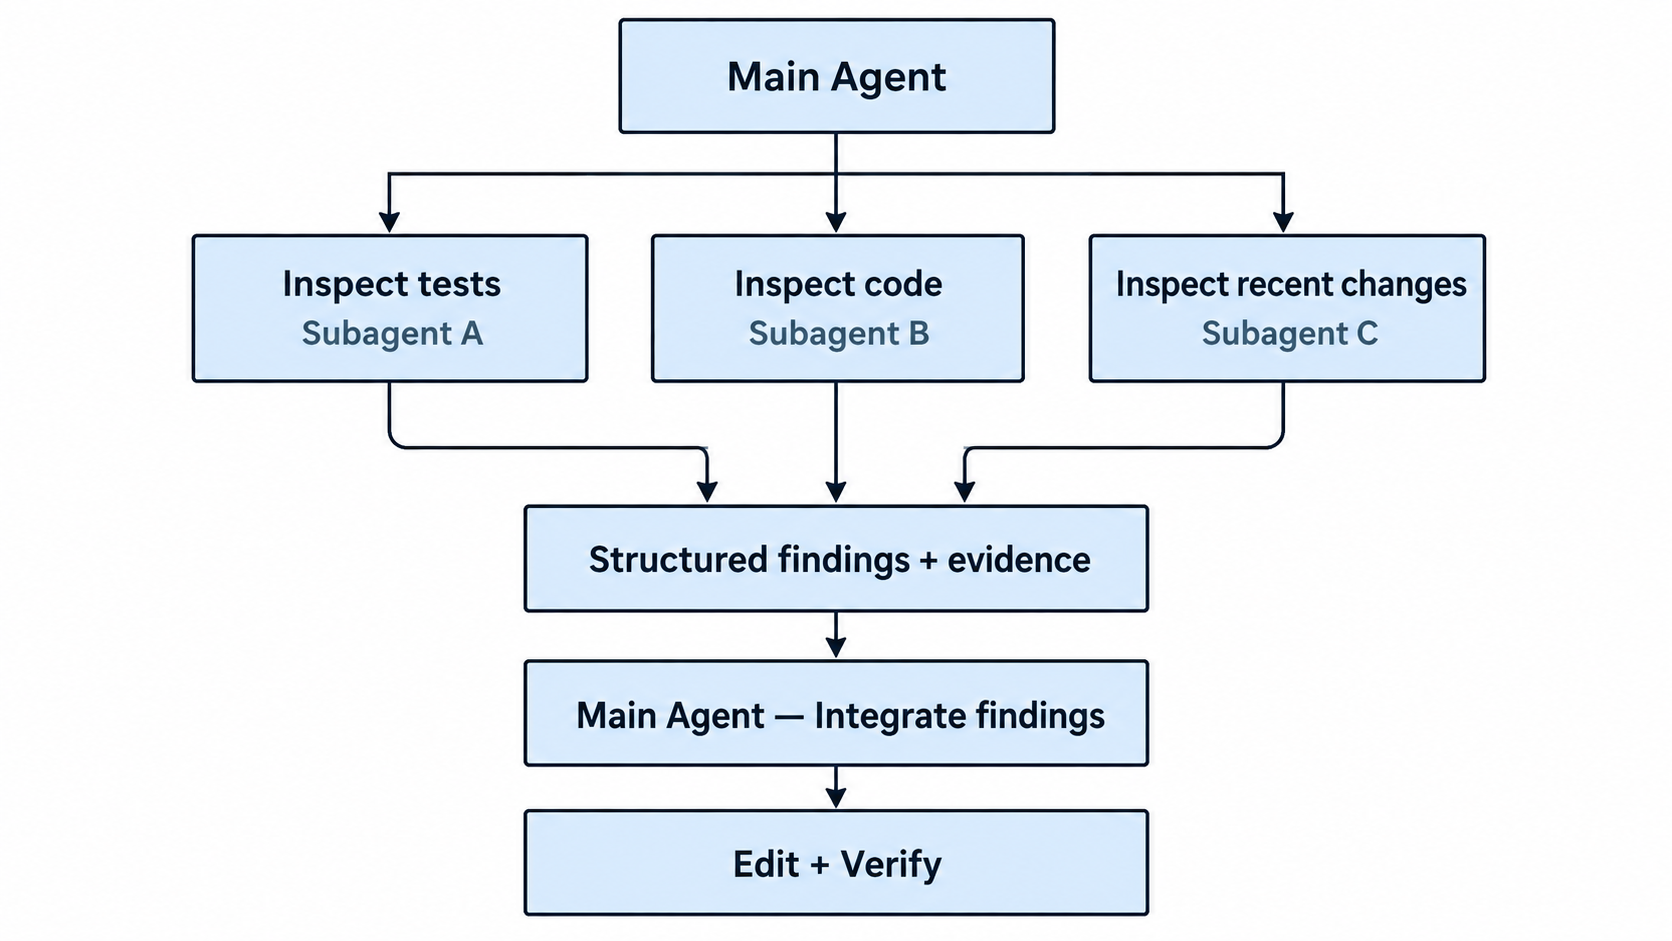
\includegraphics[width=0.88\linewidth]{images/agent-subagent-delegation.png}
\captionof{figure}{Delegation of independent investigation tasks to subagents, followed by centralised integration and verification by the main agent.}
\label{fig:agent-delegation}
\end{minipage}
\end{center}

Subagents can reduce context interference because each receives only information relevant to its task, and logically independent investigations may execute concurrently. Anthropic applies a related pattern in its multi-agent research system, where a lead agent delegates independent research directions and later combines their results \parencite{hadfield2025multiagent}.

Logical independence does not guarantee lower latency. Several subagents sharing a constrained local inference backend may compete for the same compute resources. Delegated findings should therefore be useful even without parallel speedup and retain enough provenance to identify the inspected code state and supporting observations.

Parallel modification of shared repository state creates additional coordination problems because agents may operate on outdated assumptions or produce conflicting edits. For the assistant considered here, a conservative pattern is to use subagents primarily for independent investigation while the main agent performs integration, code modification and final verification.

The harness tracks delegated work and enforces predefined failure and budget policies, while the main agent evaluates conflicting findings and decides whether further investigation is required.

Agent harnesses therefore connect model decisions, context, tools and task state into adaptive multi-step execution, while subagents add bounded delegation where useful. Deploying this execution model reliably introduces separate concerns such as model routing, long-running task persistence, resource contention and scalability, which are addressed in the following chapter.
